\documentclass{article}
\usepackage[x11names, rgb]{xcolor}
\usepackage[utf8]{inputenc}
\usepackage{tikz}
\usetikzlibrary{snakes,arrows,shapes}
\usepackage{amsmath}
% from http://www.fauskes.net/code/dot2tex/gallery/automata/
%
%
\usetikzlibrary{automata}%

\begin{document}
\pagestyle{empty}
%
%
%

\enlargethispage{100cm}
% Start of code
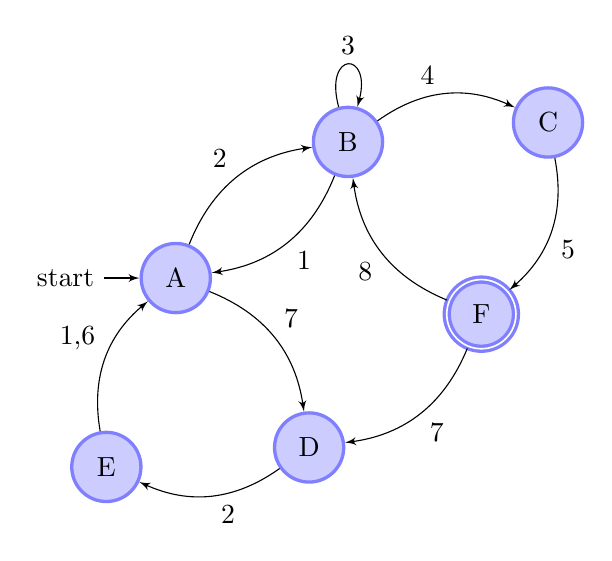
\begin{tikzpicture}[>=latex',join=bevel,]
\tikzstyle{every state}=     [draw=blue!50,very thick,fill=blue!20]%
\node (A) at (53bp,87bp) [state, initial] {A};
  \node (B) at (115bp,136bp) [state] {B};
  \node (D) at (101bp,26bp) [state] {D};
  \node (C) at (187bp,143bp) [state] {C};
  \node (F) at (163bp,74bp) [state,accepting] {F};
  \node (E) at (28bp,19bp) [state] {E};
  \draw [->] (A) to[bend left] node[auto] {2} (B);
  \draw [->] (A) to[bend left] node[auto] {7} (D);
  \draw [->] (B) to[bend left] node[auto] {1} (A);
  \draw [->] (B) to[loop above] node[auto] {3} (B);
  \draw [->] (B) to[bend left] node[auto] {4} (C);
  \draw [->] (C) to[bend left] node[auto] {5} (F);
  \draw [->] (F) to[bend left] node[auto] {8} (B);
  \draw [->] (F) to[bend left] node[auto] {7} (D);
  \draw [->] (D) to[bend left] node[auto] {2} (E);
  \draw [->] (E) to[bend left] node[auto] {1,6} (A);
%
\end{tikzpicture}
% End of code

%
\end{document}
%


